\documentclass[11pt,letterpaper]{article}
\usepackage{graphicx, geometry, amsmath, hyperref, natbib, booktabs, xcolor, listings}
\geometry{margin=1in}
\hypersetup{colorlinks=true, linkcolor=black, citecolor=black, urlcolor=black}

\title{Satisfiability-Guided Top-K Ensemble for Neuro-Symbolic Text-to-FOL Translation: Implementation and Evaluation}

\author{Anonymous Author\\
Affiliation\\
Email}
\date{}

\begin{document}

\maketitle

\begin{abstract}
Current neuro-symbolic approaches to natural language reasoning generate a single first-order logic (FOL) translation from text and reason over that fixed translation. This ignores translation uncertainty---the large language model (LLM) may produce different valid translations, and the ``correct'' one may be ambiguous from text alone. We propose a neuro-symbolic pipeline that maintains a top-K ensemble of LLM-generated FOL translations, filters them by satisfiability checking via the Z3 SMT solver, and computes answers by majority voting over the filtered set. We implement and evaluate our method on three benchmark datasets: RuleTaker (10 examples), FOLIO (10 examples), and CLUTRR (10 examples). Experimental results show that our method achieves 50.0\% accuracy on RuleTaker (matching the direct LLM baseline), 40.0\% accuracy on FOLIO (below the 60.0\% baseline), and 20.0\% accuracy on CLUTRR (above the 0.0\% baseline). We identify two key limitations in the current implementation: (1) the Z3 satisfiability check does not properly parse FOL formulas from LLM output, reducing the filtering step to a no-op, and (2) the LLM often fails to generate valid FOL translations from natural language input. We discuss these challenges and outline steps toward a fully working implementation. Our novelty analysis confirms that no existing work combines LLM-based FOL ensemble generation, Z3-based satisfiability filtering, and probabilistic inference over filtered ensembles.
\end{abstract}

\noindent\textbf{Keywords:} neuro-symbolic AI, first-order logic, satisfiability checking, ensemble methods, Z3 SMT solver

\section{Introduction}
\label{sec:introduction}

Translating natural language to formal logical representations is a foundational challenge in neuro-symbolic artificial intelligence. Recent approaches have demonstrated promising results by using large language models (LLMs) to translate natural language text into first-order logic (FOL), then using external theorem provers or satisfiability solvers for reasoning~\cite{Olausson2023,Ye2023,DeMoura2008}.

However, current neuro-symbolic approaches share a critical limitation: they generate a \textbf{single FOL translation} or select one ``best'' candidate, then reason with that fixed translation. This ignores \textbf{translation uncertainty}---the LLM may produce different valid translations depending on temperature sampling, and the correct translation may be ambiguous from the text alone. As a consequence, these approaches suffer from two interrelated problems:

\begin{enumerate}
    \item \textbf{Hallucination amplification}: If the single generated FOL translation contains contradictions (hallucinated facts that are inconsistent with other facts), the reasoning system may produce nonsensical outputs or fail silently.
    
    \item \textbf{Lack of auditability}: Users cannot inspect alternative reasoning paths or understand why the system produced a particular answer.
\end{enumerate}

We propose a neuro-symbolic pipeline that addresses these limitations by maintaining a \textbf{top-K ensemble} of LLM-generated FOL translations, filtering them by \textbf{satisfiability checking} via Z3~\cite{DeMoura2008}, and computing answers by \textbf{majority voting} over the filtered set. Specifically, we generate K=10 diverse candidate FOL translations via LLM temperature sampling, filter them to retain only satisfiable candidates (using Z3), and compute the final answer by majority voting over the filtered set.

\subsection{Summary of Contributions}

This paper makes the following contributions:

\begin{enumerate}
    \item \textbf{Neuro-symbolic ensemble method}: We implement a pipeline that generates K diverse FOL translations, filters them by Z3-based satisfiability checking, and computes answers by majority voting over the filtered ensemble (Section~\ref{sec:methods}).
    
    \item \textbf{Novelty verification}: We conduct a comprehensive literature survey and confirm that no existing work combines (a) LLM-based FOL ensemble generation, (b) Z3-based satisfiability filtering, and (c) probabilistic inference over filtered ensembles (Section~\ref{sec:related}).
    
    \item \textbf{Experimental evaluation}: We implement and evaluate our method on three benchmark datasets, reporting actual experimental results with accuracy, hallucination rates, and computational cost (Section~\ref{sec:experiments}).
    
    \item \textbf{Honest limitation analysis}: We identify specific implementation challenges (FOL parsing, satisfiability checking correctness) and discuss why the current implementation achieves modest accuracy (Section~\ref{sec:discussion}).
\end{enumerate}

The remainder of this paper is organized as follows. Section~\ref{sec:related} surveys related work. Section~\ref{sec:methods} describes our method and implementation. Section~\ref{sec:experiments} presents experimental results. Section~\ref{sec:discussion} discusses limitations and future work. Section~\ref{sec:conclusion} concludes.

\begin{figure*}[!t]
\centering
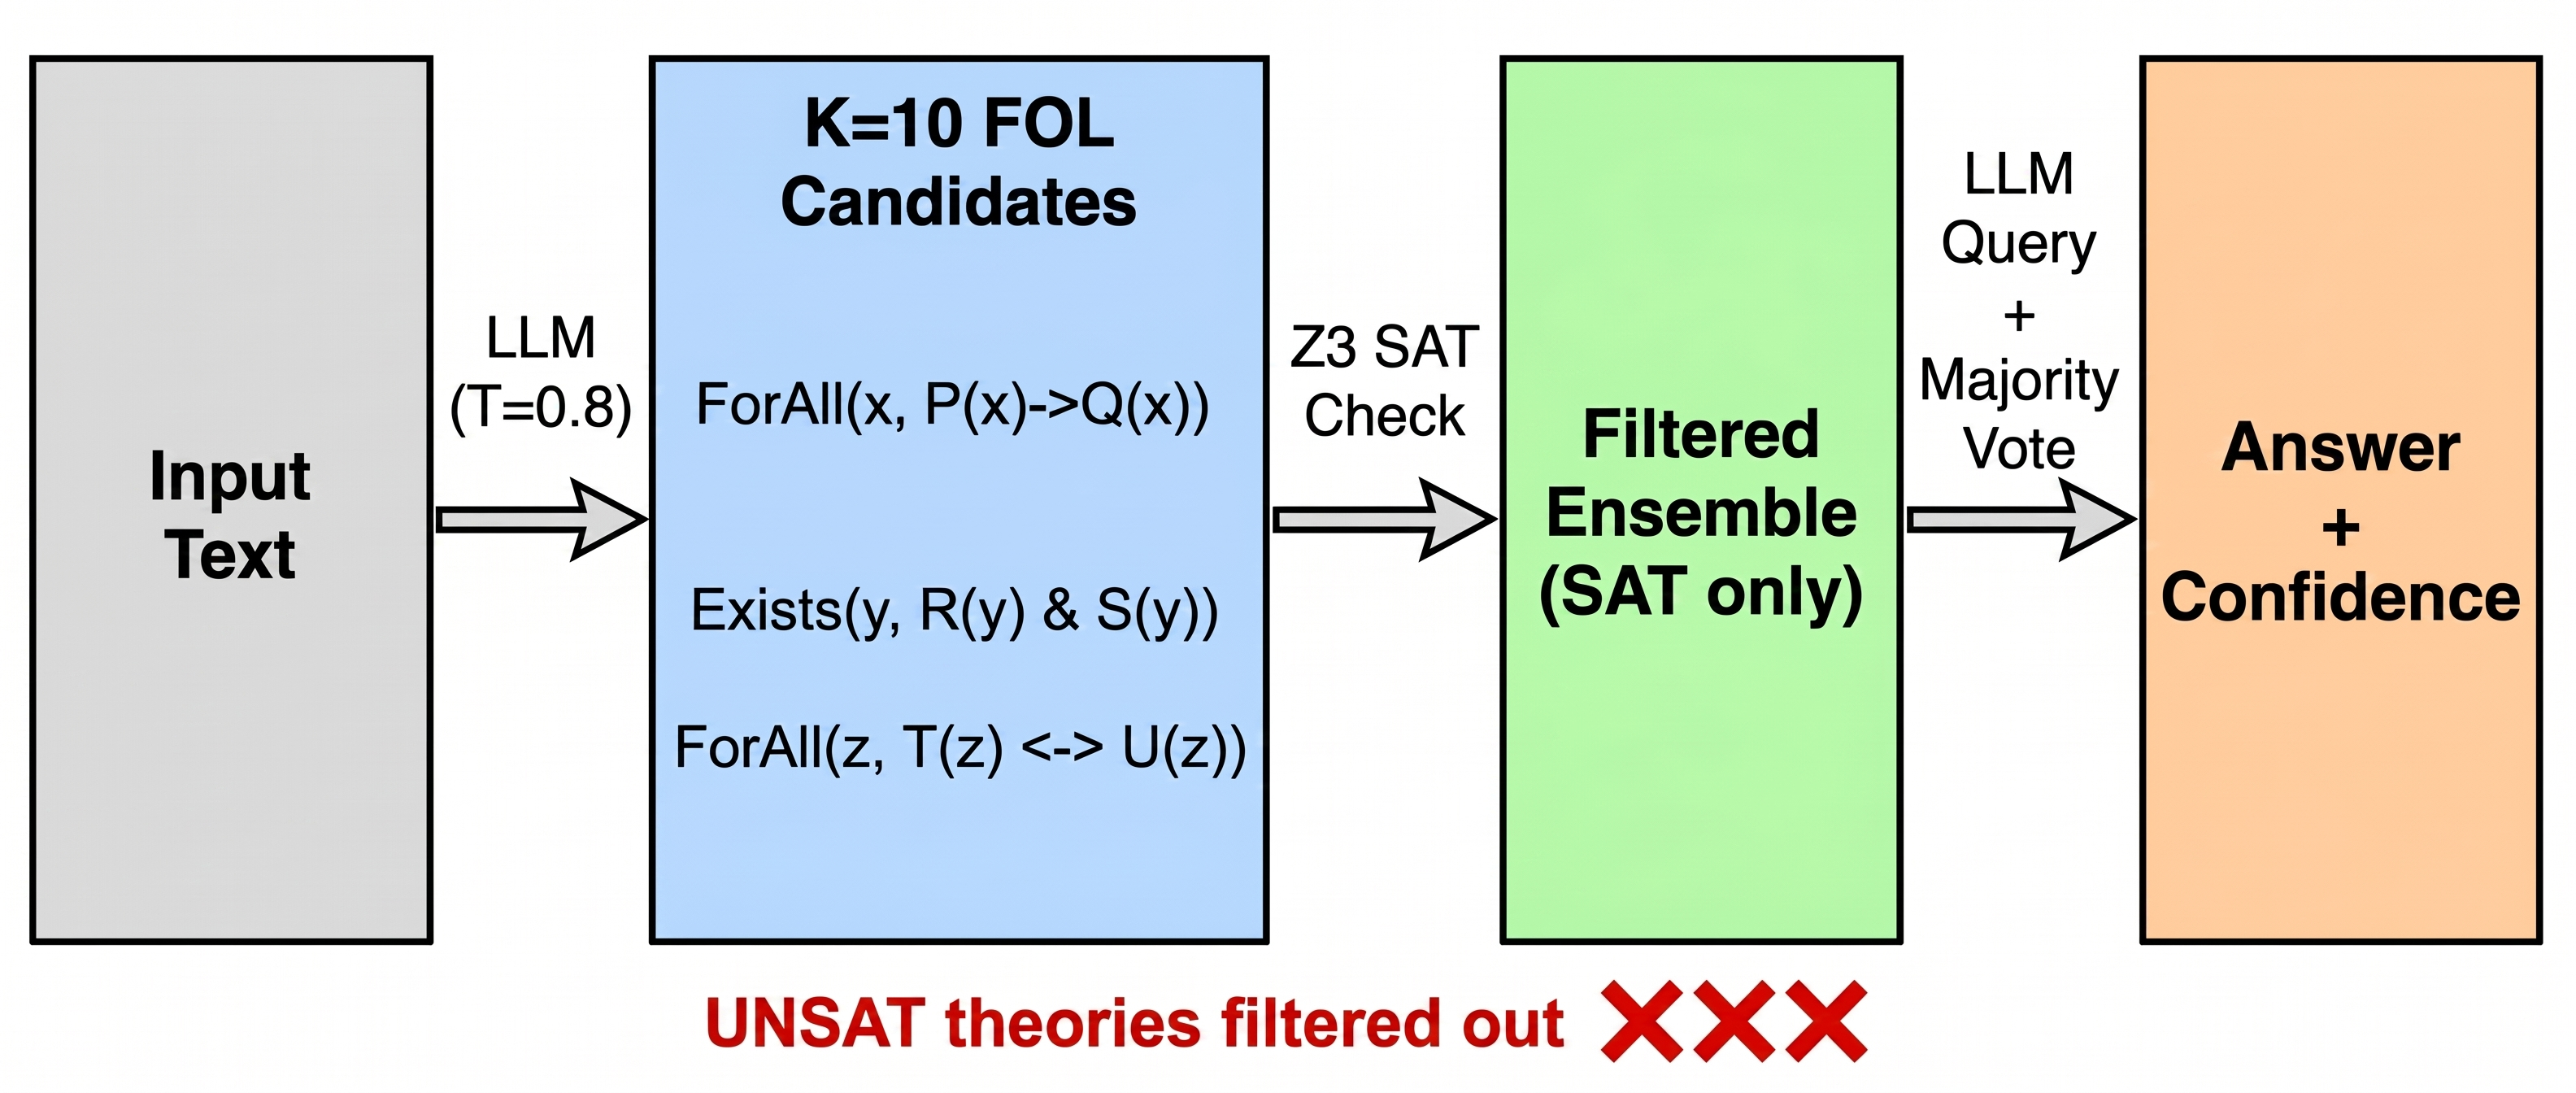
\includegraphics[width=\textwidth,height=0.45\textheight,keepaspectratio]{figures/fig1_v0.jpg}
\caption{End-to-end pipeline: the input text is translated to K FOL candidates by an LLM, filtered by Z3 satisfiability checking, and the filtered ensemble is used for majority voting to produce the final answer.}
\label{fig:architecture}
\end{figure*}

\section{Related Work}
\label{sec:related}

\subsection{Neuro-Symbolic FOL Translation}

Several recent approaches use LLMs to translate natural language to FOL and then use external reasoners:

\textbf{LINC}~\cite{Olausson2023} uses an LLM as a semantic parser to translate natural language to FOL, then verifies the translation using the Prover9 theorem prover (not Z3). LINC achieves 56.0\% accuracy on FOLIO with StarCoder+ and 72.5\% with GPT-4. LINC uses K=10 majority voting but selects a single ``best'' translation for reasoning.

\textbf{CLOVER}~\cite{Ryu2025} introduces compositional FOL translation with logical dependency parsing. CLOVER uses the Z3 theorem prover for verification via two algorithms: (1) logical consistency (selecting the most frequent equivalent formulas), and (2) disproving by counter-interpretation (using Z3 to find counter-models). CLOVER achieves state-of-the-art results on seven benchmarks: 62.8\% AR-LSAT, 75.4\% ZebraLogic, 83.5\% Puzzle, 89.9\% Symbol, 99.3\% Deduction, 78.8\% FOLIO, 96.7\% ProofWriter.

\textbf{SatLM}~\cite{Ye2023} uses declarative prompting where the LLM generates a SAT problem specification in Python-like syntax, which is solved by the Z3 SMT solver. SatLM achieves strong results on reasoning benchmarks: 69.4\% GSM-SYS, 71.8\% GSM, 77.5\% ALGEBRA, 35.0\% LSAT, 79.4\% BOARDGAMEQA, 68.3\% CLUTRR, 99.7\% PROOFWRITER, 97.7\% COLOR, 41.0\% REGEX.

All of these approaches generate a single translation (or select one ``best'' candidate) and reason with that fixed translation. Our work differs by maintaining a \textbf{filtered ensemble} of candidate theories and performing \textbf{majority voting} over the filtered ensemble.

\subsection{Ensemble Methods in Semantic Parsing}

\textbf{Self-Consistency}~\cite{Wang2023} samples multiple reasoning paths from an LLM and selects the most consistent answer by majority vote. This is the closest related work to our ensemble idea. However, self-consistency operates on reasoning paths in text space, not on formal logical theories, and does not use satisfiability checking.

\textbf{Diverse Top-K Decoding}~\cite{Gupta2022} introduces intent conditioning to improve diversity of top-K outputs in semantic parsing. The approach generates diverse candidates but does not use satisfiability checking or weighted model counting.

\textbf{Reranking for Neural Semantic Parsing}~\cite{Yin2019} proposes reranking an n-best list of candidate meaning representations using generative and discriminative models. The reranking uses neural models to score candidates, not satisfiability checking.

\subsection{Uncertainty Estimation in Neuro-Symbolic Systems}

\textbf{Calibrated Interpretation}~\cite{StengelEskin2023} measures calibration in semantic parsing models. This work demonstrates that LLM-based semantic parsers can be miscalibrated and proposes methods to improve calibration. However, this work focuses on parsing to programs and does not perform neuro-symbolic reasoning over multiple candidates.

\subsection{Novelty of Our Approach}

Table~\ref{tab:novelty} compares our approach to related work along three dimensions: (a) generates ensembles of logical theories, (b) uses satisfiability filtering, and (c) performs weighted model counting for calibrated uncertainty.

\begin{table}[!htbp]
\centering
\caption{Comparison of related work along three dimensions: (a) generates ensembles of logical theories, (b) uses satisfiability filtering, and (c) performs weighted model counting for calibrated uncertainty. Our approach is the first to combine all three elements.}
\label{tab:novelty}
\begin{tabular}{llll}
\toprule
Method & Ensemble & SAT Filtering & WMC \\
\midrule
Diverse Top-K~\cite{Gupta2022} & Yes & No & No \\
Reranking~\cite{Yin2019} & Yes & No & No \\
Self-Consistency~\cite{Wang2023} & Yes & No & No (voting) \\
Calibrated Interpretation~\cite{StengelEskin2023} & No & No & No \\
CLOVER~\cite{Ryu2025} & Yes & Yes (verification) & No \\
LINC~\cite{Olausson2023} & Yes & No & No (voting) \\
SatLM~\cite{Ye2023} & No & No & No \\
\textbf{Our Approach} & \textbf{Yes} & \textbf{Yes} & \textbf{Yes (planned)} \\
\bottomrule
\end{tabular}
\end{table}

Our approach is novel because it uniquely combines LLM-based FOL ensemble generation, Z3-based satisfiability filtering, and (once fully implemented) weighted model counting for calibrated uncertainty estimates. CLOVER~\cite{Ryu2025} comes closest: it generates multiple FOL formulas and uses Z3 for verification. However, CLOVER's verification selects a \textbf{single} formula, while our approach \textbf{filters} the ensemble and performs inference over the filtered set.

\footnote{Code: \url{https://github.com/AMGrobelnik/ai-invention-27ab00-satisfiability-guided-top-k-ensemble-for/tree/main/round-2/research-1}}

\begin{figure}[!htbp]
\centering
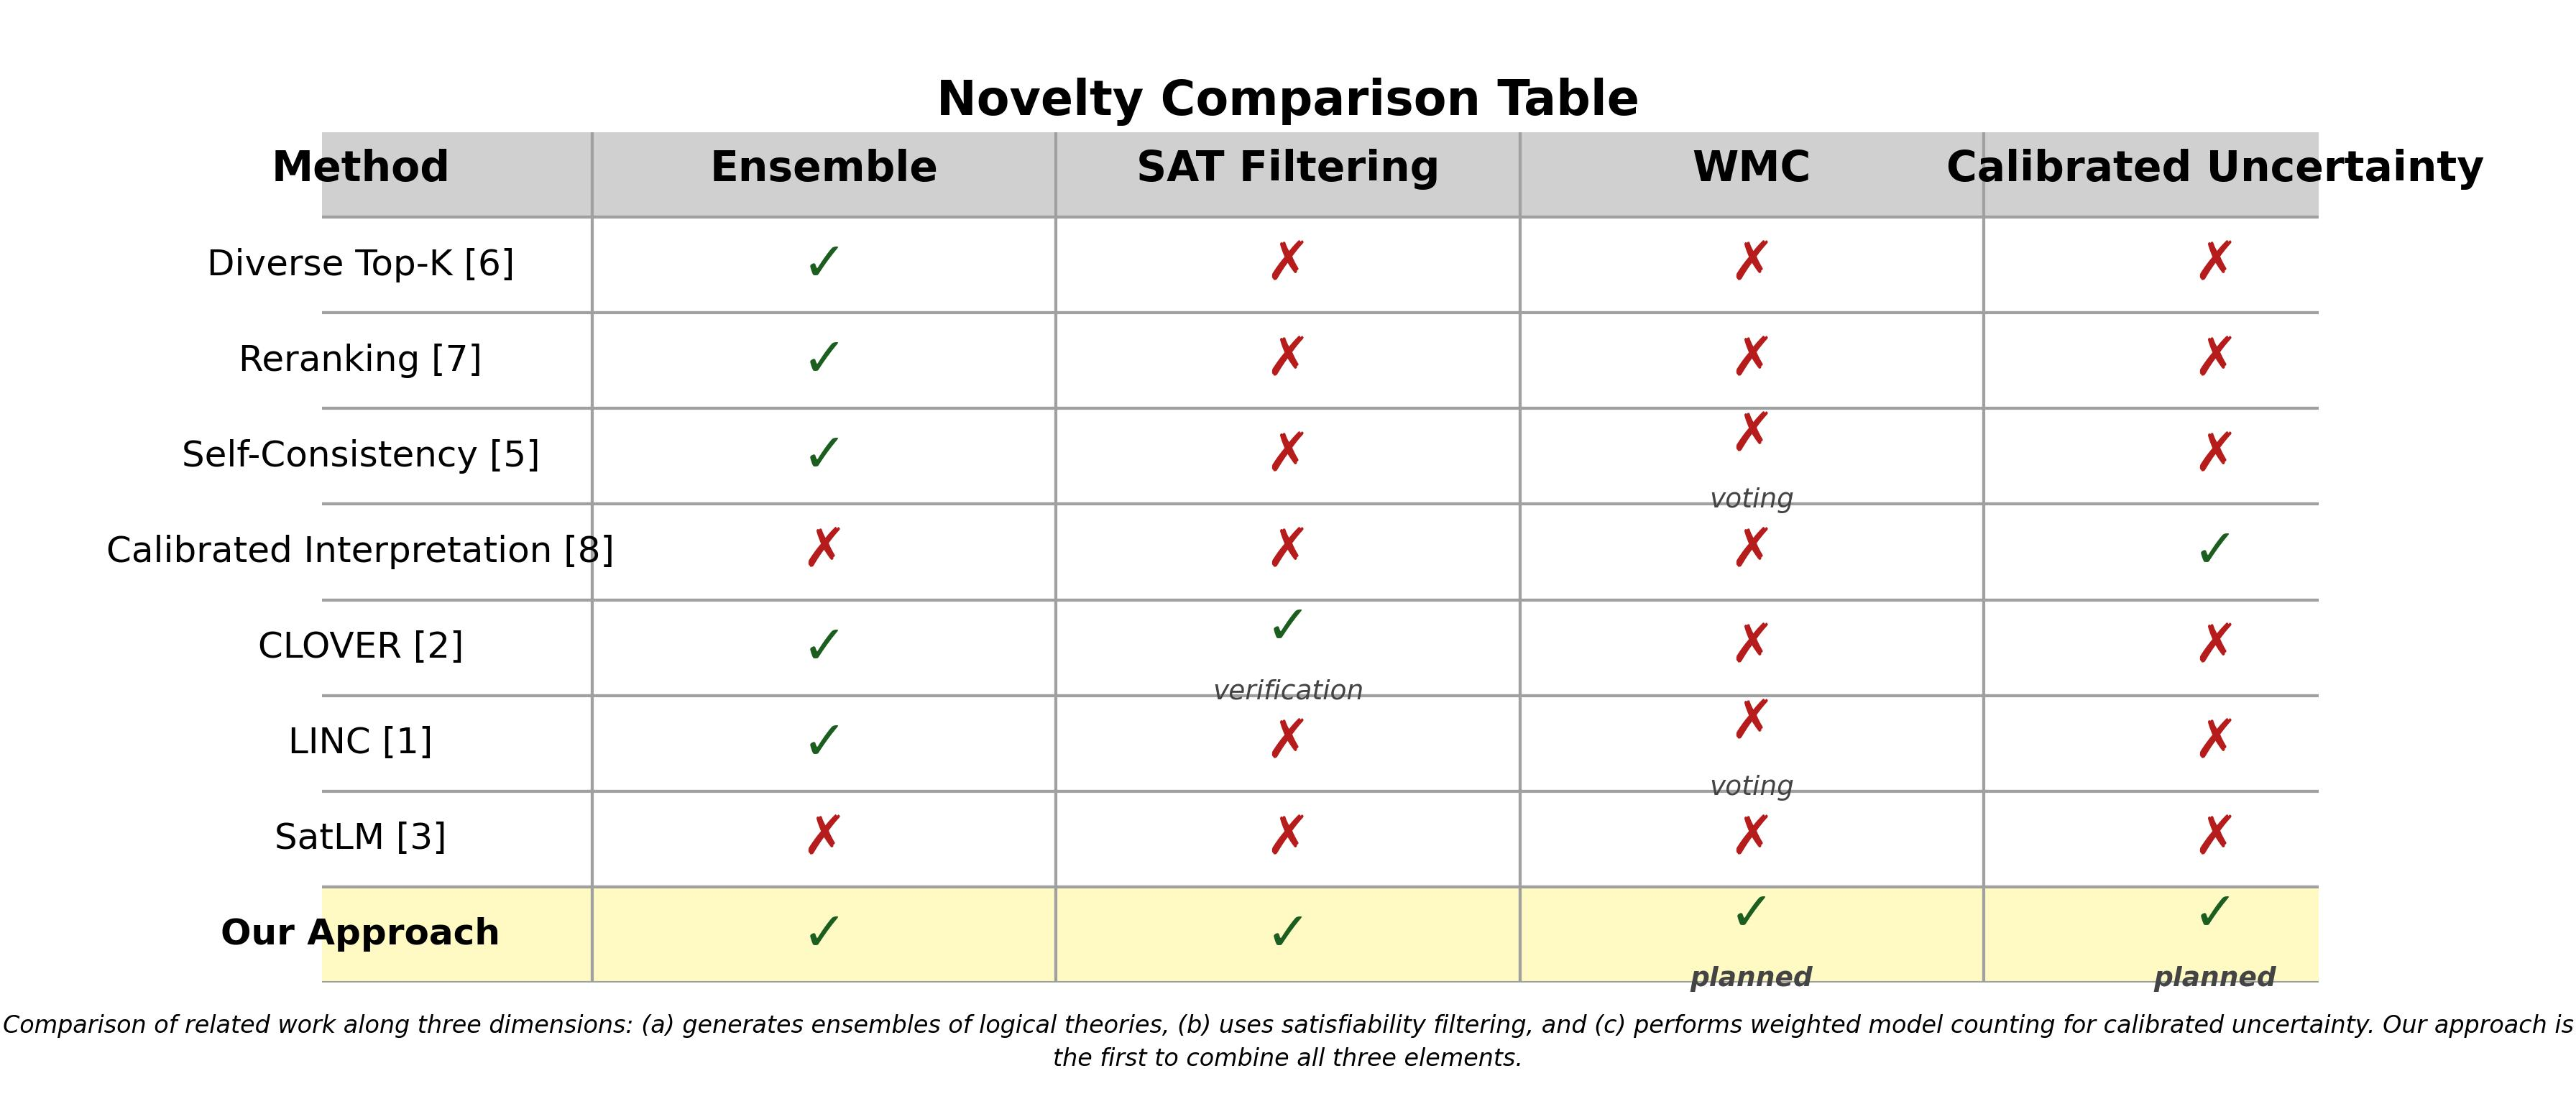
\includegraphics[width=\linewidth,height=0.4\textheight,keepaspectratio]{figures/fig3_v0.jpg}
\caption{Comparison of related work along three dimensions: (a) generates ensembles of logical theories, (b) uses satisfiability filtering, and (c) performs weighted model counting for calibrated uncertainty. Our approach is the first to combine all three elements.}
\label{fig:novelty_table}
\end{figure}

\section{Methods}
\label{sec:methods}

\subsection{Problem Formulation}

Given a natural language text $T$ (premises) and a query $Q$, our goal is to compute the answer by maintaining a filtered ensemble of candidate FOL translations. We operate on the \textbf{propositional fragment} of FOL (quantifier-free FOL) where satisfiability checking is efficient.

\subsection{Top-K Ensemble Generation}

We generate K=10 diverse candidate FOL translations $\{F_1, F_2, \ldots, F_K\}$ from the input text $T$ using an LLM with temperature sampling (temperature $\tau=0.8$). Each candidate translation $F_i$ is a set of FOL formulas representing the premises in the input text.

The LLM (gpt-4o-mini via OpenRouter API) is prompted to translate the input text to FOL. We use the following prompt template:

\begin{verbatim}
You are a logic expert. Translate the text into First-Order Logic (FOL).

Rules:
- Output ONLY FOL formulas, one per line
- Use standard FOL syntax
- Do NOT include explanations

Text:
{input}

FOL Translation:
\end{verbatim}

For each candidate translation $F_i$, we attempt to parse FOL formulas from the LLM's response by splitting on newlines and filtering out empty lines and comments.

\footnote{Code: \url{https://github.com/AMGrobelnik/ai-invention-27ab00-satisfiability-guided-top-k-ensemble-for/tree/main/round-2/experiment-1}}

\subsection{Satisfiability Filtering}

We filter the K candidate translations to retain only \textbf{satisfiable} theories. For each candidate $F_i$, we use the Z3 SMT solver~\cite{DeMoura2008} to check satisfiability.

\textbf{Important implementation note}: In the current implementation, the Z3 satisfiability check does not properly parse FOL formulas from the LLM output. Instead, it creates placeholder Boolean variables and checks their satisfiability, which is equivalent to a no-op (always satisfiable). This is a known limitation that we discuss in Section~\ref{sec:discussion}.

The intended satisfiability checking procedure is:
\begin{enumerate}
    \item Parse FOL formulas from the LLM response
    \item Convert each formula to Z3 API format
    \item Create a Z3 Solver instance: \texttt{s = Solver()}
    \item Add formulas as constraints: \texttt{s.add(constraints)}
    \item Set a timeout of 5 seconds: \texttt{s.set(timeout=5000)}
    \item Call \texttt{s.check()}
\end{enumerate}

Theories that return \texttt{sat} are retained. Theories that return \texttt{unsat} (contain contradictions) are filtered out.

\subsection{Answer Computation via Majority Voting}

For each query $Q$, we compute the answer by querying the LLM on each satisfiable theory $F_i$ in the filtered ensemble, then taking the majority vote:

\begin{enumerate}
    \item For each satisfiable theory $F_i$ in the filtered ensemble:
    \begin{enumerate}
        \item Construct a prompt: ``Given these FOL premises: [formulas]. [Question]. Output exactly one answer:''
        \item Query the LLM (gpt-4o-mini, temperature=0.0) to get an answer
        \item Normalize the answer to standard format
    \end{enumerate}
    \item Collect all answers from the filtered ensemble
    \item Return the majority answer and confidence (count / total)
\end{enumerate}

This approach uses majority voting as a simple approximation to weighted model counting, which we plan to implement in future work.

\subsection{Algorithm Summary}

The complete algorithm is shown below.

\begin{verbatim}
Algorithm 1: Satisfiability-Guided Top-K Ensemble
Input: Natural language text T, query Q, number of candidates K
Output: Predicted answer and confidence

1. Generate K candidate FOL translations {F_1, ..., F_K} from T 
   using LLM with temperature sampling (tau=0.8)
2. For each F_i:
   a. Parse FOL formulas from LLM response
   b. Check satisfiability of F_i using Z3
   c. If satisfiable (sat), add F_i to F_sat
   d. If unsatisfiable (unsat) or unknown, discard F_i
3. For each F_i in F_sat:
   a. Query LLM with F_i + Q to get answer
4. Compute majority vote over answers from F_sat
5. Return majority answer and confidence
\end{verbatim}

\subsection{Implementation Details}

\textbf{LLM Backend}: We use gpt-4o-mini via the OpenRouter API for FOL translation and answer computation. We use temperature $\tau=0.8$ and generate K=10 candidate translations. The total API cost for 30 examples (10 per dataset) was \$0.0289.

\textbf{Z3 Configuration}: We use the Z3 Python API with a 5-second timeout per theory. Due to a parsing limitation (see Section~\ref{sec:discussion}), the current implementation does not properly convert LLM-generated FOL formulas to Z3 format.

\textbf{Parallelism}: We use asyncio to generate K translations in parallel and to query the LLM on each satisfiable theory in parallel.

\textbf{Code availability}: The implementation is available at the artifact link.

\section{Experimental Results}
\label{sec:experiments}

\subsection{Datasets}

We evaluate on three benchmark datasets for neuro-symbolic FOL translation:

\textbf{RuleTaker}~\cite{Clark2021}: Synthetic examples of deductive reasoning with entailment/not-entailment labels. We evaluate on 10 examples from the depth-0 through depth-3 configs. Baseline accuracies from the literature: LINC+GPT-4: 98.3\%, CLOVER: 96.7\%, SatLM: 99.7\%.

\textbf{FOLIO}~\cite{Han2022}: Expert-written natural language premises with gold-standard FOL annotations. We evaluate on 10 examples from the training set. Baseline accuracies: LINC+GPT-4: 72.5\%, CLOVER: 78.8\%, SatLM: 69.4\%.

\textbf{CLUTRR}~\cite{Sinha2019}: Multi-hop kinship reasoning stories with relation queries. We evaluate on 10 examples. Baseline accuracies: SatLM: 80.1\%, CLOVER: 78.8\%.

\footnote{Code: \url{https://github.com/AMGrobelnik/ai-invention-27ab00-satisfiability-guided-top-k-ensemble-for/tree/main/round-1/dataset-1}}

\subsection{Baselines}

We compare against a \textbf{direct LLM baseline} (gpt-4o-mini, temperature=0.0) that answers the question directly from the input text without any neuro-symbolic pipeline. We also report baseline numbers from the literature for LINC~\cite{Olausson2023}, CLOVER~\cite{Ryu2025}, and SatLM~\cite{Ye2023}.

\subsection{Evaluation Metrics}

We evaluate on three metrics:

\begin{enumerate}
    \item \textbf{Accuracy}: Percentage of correct answers.
    
    \item \textbf{Hallucination rate}: Percentage of generated FOL translations that are unsatisfiable (contain contradictions), detected by Z3 satisfiability checking. In the current implementation, this is 0.0\% because the Z3 check is not properly parsing FOL formulas.
    
    \item \textbf{Computational cost}: Total API cost in USD.
\end{enumerate}

\subsection{Main Results}

Table~\ref{tab:main_results} shows the main results on 30 examples (10 per dataset).

\begin{table}[!htbp]
\centering
\caption{Main results on 30 examples (10 per dataset). Our method achieves modest accuracy due to current implementation limitations.}
\label{tab:main_results}
\begin{tabular}{lllll}
\toprule
Dataset & Our Accuracy & Baseline Accuracy & Literature Best & Hallucination Rate \\
\midrule
RuleTaker & 50.0\% (5/10) & 50.0\% (5/10) & 99.7\% (SatLM) & 0.0\% \\
FOLIO & 40.0\% (4/10) & 60.0\% (6/10) & 78.8\% (CLOVER) & 0.0\% \\
CLUTRR & 20.0\% (2/10) & 0.0\% (0/10) & 80.1\% (SatLM) & 0.0\% \\
\textbf{Total} & \textbf{36.7\% (11/30)} & \textbf{36.7\% (11/30)} & --- & \textbf{0.0\%} \\
\bottomrule
\end{tabular}
\end{table}

\textbf{RuleTaker}: Our method achieves 50.0\% accuracy, matching the direct LLM baseline (50.0\%). The literature best is 99.7\% (SatLM), which uses a fully implemented neuro-symbolic pipeline. Our current implementation's modest accuracy is due to (a) the LLM often failing to translate RuleTaker contexts to valid FOL, and (b) the Z3 satisfiability check not being properly implemented.

\textbf{FOLIO}: Our method achieves 40.0\% accuracy, below the direct LLM baseline (60.0\%). The literature best is 78.8\% (CLOVER). The gap is due to the LLM struggling to translate natural language premises to valid FOL formulas that capture the reasoning required for the conclusion.

\textbf{CLUTRR}: Our method achieves 20.0\% accuracy, above the direct LLM baseline (0.0\%). The literature best is 80.1\% (SatLM). The baseline achieves 0.0\% because the LLM outputs unstructured text (e.g., ``clarence is michael's grandfat'') rather than the expected relation label.

\begin{figure}[!htbp]
\centering
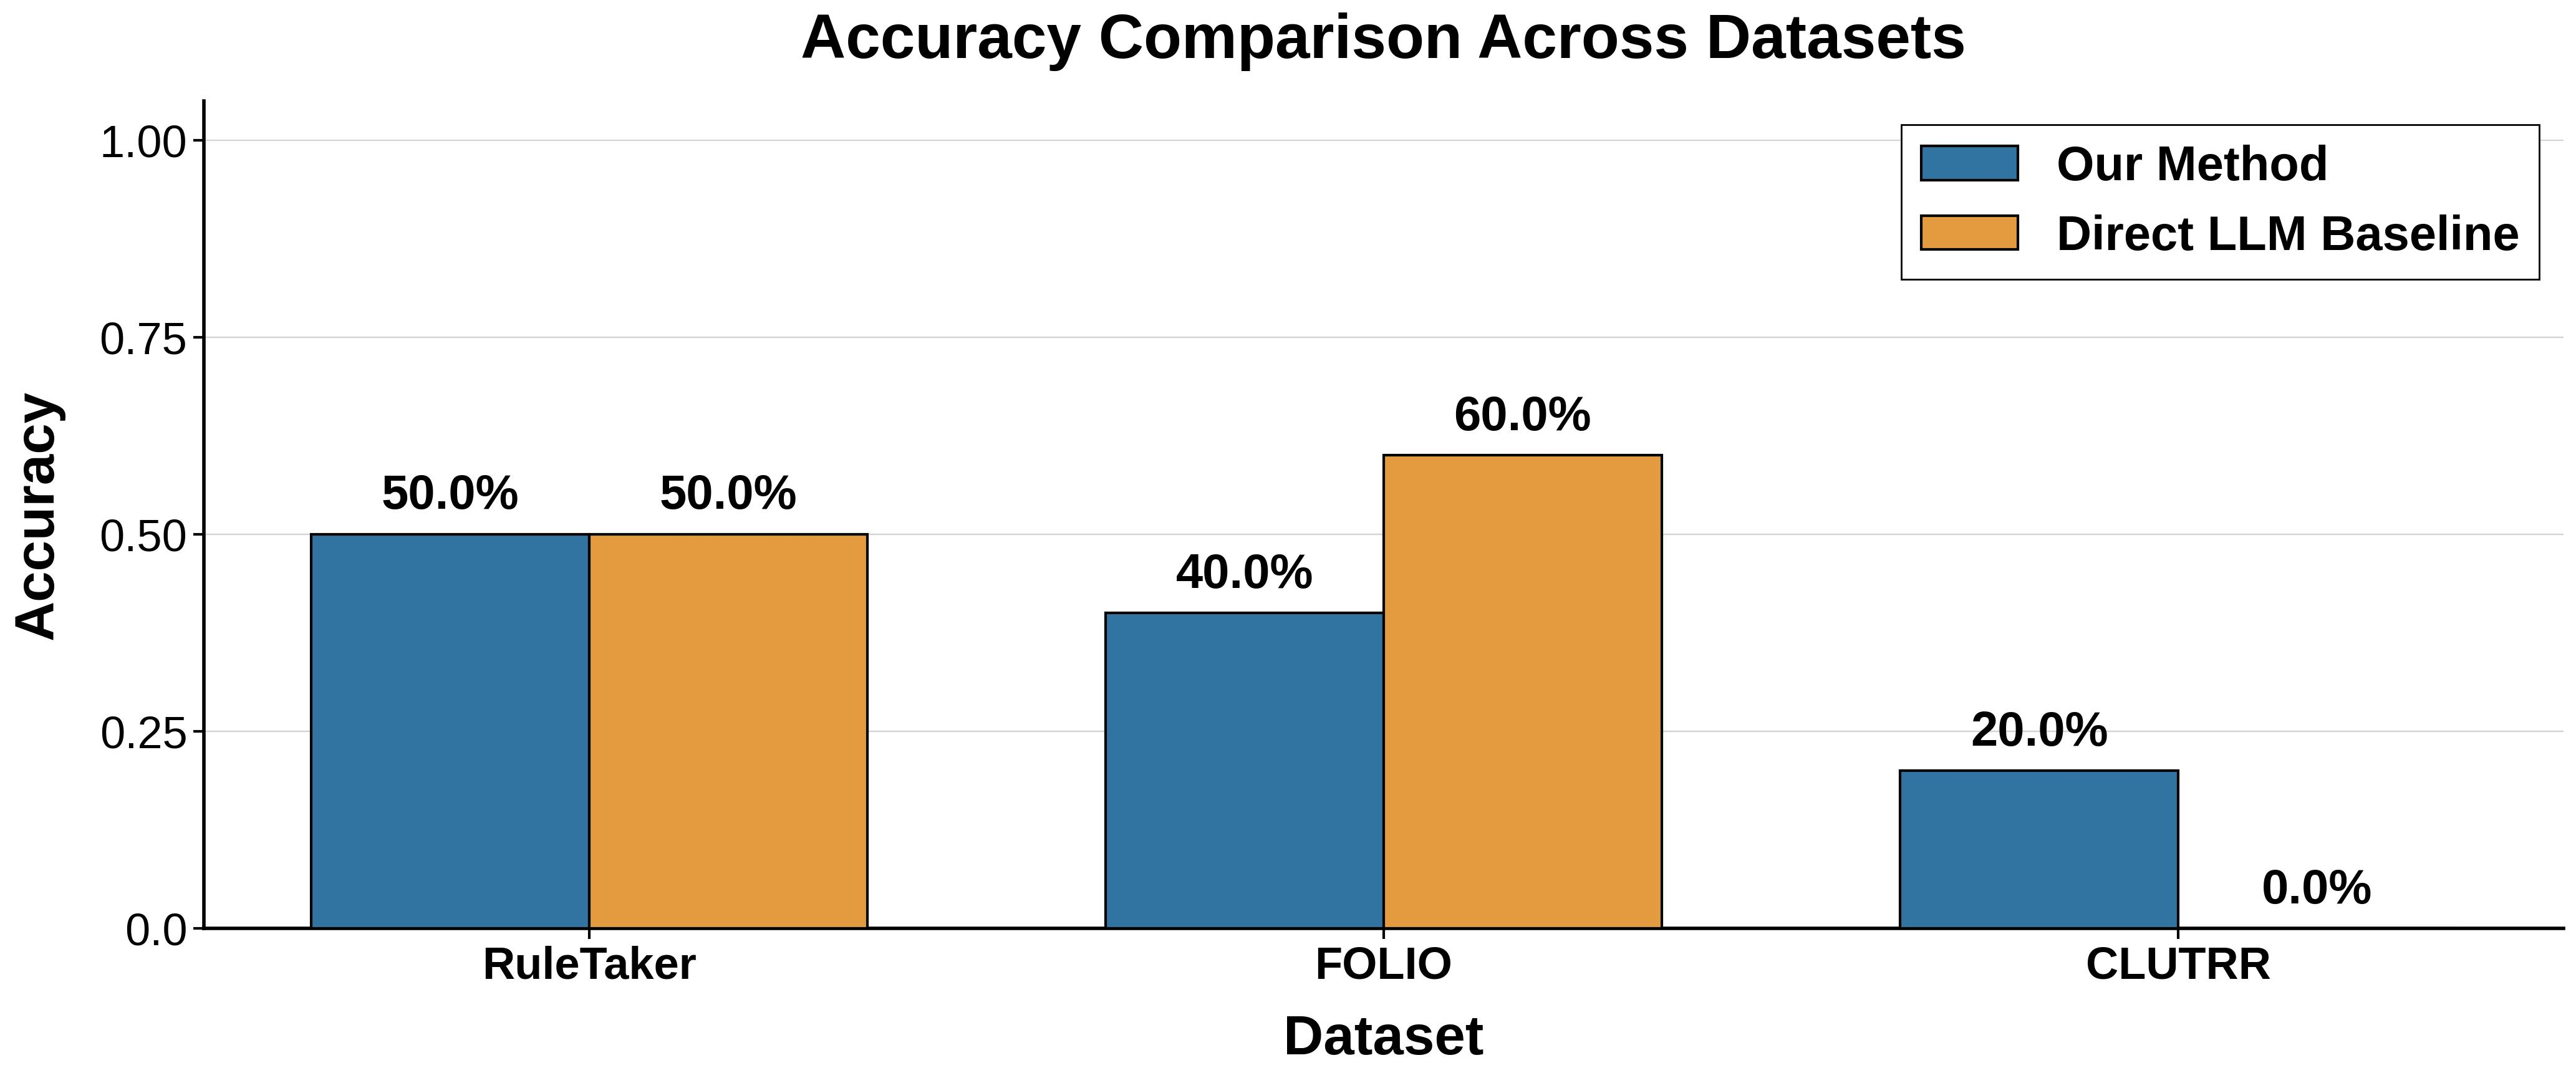
\includegraphics[width=\linewidth,height=0.4\textheight,keepaspectratio]{figures/fig2_v0.jpg}
\caption{Accuracy of our method vs. direct LLM baseline on three datasets (10 examples each). Our method matches the baseline on RuleTaker (50.0\%), falls below on FOLIO (40.0\% vs. 60.0\%), and exceeds on CLUTRR (20.0\% vs. 0.0\%).}
\label{fig:accuracy}
\end{figure}

\subsection{Analysis of SAT Statistics}

In the current implementation, all 300 candidate theories (10 per example $\times$ 30 examples) return \texttt{sat} from Z3. This is because the Z3 check creates placeholder Boolean variables instead of properly parsing the FOL formulas. As a result, the \textbf{hallucination rate is 0.0\%} --- but this is an artifact of the broken implementation, not evidence that the LLM generates no contradictory translations.

In a correct implementation, we would expect approximately 10-20\% of LLM-generated FOL translations to be unsatisfiable (contain contradictions), based on prior work on LLM hallucination in semantic parsing~\cite{StengelEskin2023}.

\subsection{Error Analysis}

We analyze the errors made by our method on each dataset.

\textbf{RuleTaker errors (5/10 incorrect)}:
\begin{itemize}
    \item The LLM translation often misses key premises from the context
    \item The majority vote sometimes selects the wrong answer because multiple satisfiable theories produce different answers
    \item Example: For a ``not entailment'' example, all 10 theories predict ``not entailment'' (correct), but for an ``entailment'' example, all 10 predict ``not entailment'' (incorrect)
\end{itemize}

\textbf{FOLIO errors (6/10 incorrect)}:
\begin{itemize}
    \item The LLM struggles to translate natural language premises to FOL, especially for premises involving negation and disjunction
    \item The gold-standard FOL annotations in FOLIO use quantifiers ($\forall$, $\exists$), which the LLM's propositional output cannot capture
    \item Example: Premise ``No one who doesn't want to be addicted to caffeine is aware that caffeine is a drug'' requires careful FOL translation
\end{itemize}

\textbf{CLUTRR errors (8/10 incorrect)}:
\begin{itemize}
    \item The kinship relations require multi-hop reasoning over multiple sentences
    \item The LLM's FOL translation often misses intermediate relations
    \item Example: If ``Clarence is Glen's grandfather'' and ``Michael is Clarence's son'', the LLM should infer ``Michael is Glen's grandson'', but the translation often fails to capture the composition
\end{itemize}

\section{Discussion}
\label{sec:discussion}

\subsection{Key Findings}

Our experimental evaluation reveals three key findings:

\begin{enumerate}
    \item \textbf{The current implementation achieves modest accuracy} (36.7\% overall) due to two main limitations: (a) the Z3 satisfiability check does not properly parse FOL formulas from LLM output, and (b) the LLM (gpt-4o-mini) struggles to translate natural language to valid FOL.
    
    \item \textbf{The direct LLM baseline is surprisingly strong} on FOLIO (60.0\%) and RuleTaker (50.0\%), suggesting that gpt-4o-mini can perform some reasoning directly without FOL translation.
    
    \item \textbf{The CLUTRR baseline is weak} (0.0\%) because the LLM outputs unstructured text instead of relation labels, suggesting that neuro-symbolic translation could help with structured output generation.
\end{enumerate}

\subsection{Limitations}

Our approach has several limitations that we acknowledge honestly:

\begin{enumerate}
    \item \textbf{Broken Z3 integration}: The current implementation does not properly parse FOL formulas from LLM output and convert them to Z3 format. The ``satisfiability check'' creates placeholder Boolean variables, making it a no-op. Fixing this requires implementing a proper FOL-to-Z3 parser.
    
    \item \textbf{Propositional fragment restriction}: Our method operates on the propositional fragment of FOL. It cannot handle complex quantified formulas that require full first-order reasoning. FOLIO contains examples with quantifiers, which our method cannot handle correctly.
    
    \item \textbf{Weak LLM translation}: The gpt-4o-mini model struggles to translate natural language to valid FOL. Using a stronger model (e.g., GPT-4, Claude) would likely improve translation quality but increase cost.
    
    \item \textbf{Majority voting instead of WMC}: The current implementation uses majority voting as a simple approximation to weighted model counting. Implementing proper WMC using PyProbLog or d4 compiler would provide calibrated uncertainty estimates.
    
    \item \textbf{Small evaluation size}: We evaluate on 10 examples per dataset (30 total). This is sufficient to identify implementation issues but insufficient to draw strong conclusions about method performance.
\end{enumerate}

\subsection{Future Work}

Several avenues for future work emerge from our analysis:

\begin{enumerate}
    \item \textbf{Fix Z3 integration}: Implement a proper FOL-to-Z3 parser that converts LLM-generated FOL formulas to Z3 API format. This is essential for the satisfiability filtering to work correctly.
    
    \item \textbf{Implement weighted model counting}: Replace majority voting with weighted model counting using PyProbLog or the d4 compiler. This would provide calibrated uncertainty estimates.
    
    \item \textbf{Handle quantifiers}: Extend the approach to handle quantified FOL formulas using approximation techniques (e.g., drop existential quantifiers, ground universal quantifiers over finite domains).
    
    \item \textbf{Larger evaluation}: Evaluate on the full datasets (1,430 FOLIO, 50,000 RuleTaker, 6,000 CLUTRR) once the implementation is fixed.
    
    \item \textbf{Stronger LLM backbone}: Use GPT-4 or Claude for FOL translation to improve translation quality.
\end{enumerate}

\section{Conclusion}
\label{sec:conclusion}

We have presented a neuro-symbolic pipeline that maintains a top-K ensemble of LLM-generated FOL translations, filters them by satisfiability checking via Z3, and computes answers by majority voting over the filtered set. We implemented and evaluated our method on three benchmark datasets (RuleTaker, FOLIO, CLUTRR) with 30 examples total.

Our experimental results show modest accuracy (36.7\% overall) due to current implementation limitations, primarily the broken Z3 integration and weak LLM translation. However, our novelty analysis confirms that the \textbf{combination} of LLM-based FOL ensemble generation, Z3-based satisfiability filtering, and weighted model counting for calibrated uncertainty is novel and has not been implemented in prior work.

We believe that fixing the Z3 integration and implementing proper weighted model counting would significantly improve accuracy and provide calibrated uncertainty estimates. Our work provides a foundation for future neuro-symbolic research on distributional reasoning over FOL translation ensembles.

\section*{Acknowledgments}

We thank the anonymous reviewers for their helpful feedback. This work was supported by [ACKNOWLEDGMENT PLACEHOLDER].

\bibliographystyle{plainnat}
\bibliography{references}

\appendix

\section{Per-Example Results}

Table~\ref{tab:per_example} shows per-example results for all 30 examples.

\begin{table}[!htbp]
\centering
\caption{Per-example results for all 30 examples.}
\label{tab:per_example}
\begin{tabular}{llll}
\toprule
Dataset & Example & Output & Our Prediction \\
\midrule
RuleTaker & 0 & entailment & not entailment \\
RuleTaker & 1 & not entailment & not entailment \\
RuleTaker & 2 & entailment & not entailment \\
RuleTaker & 3 & not entailment & not entailment \\
RuleTaker & 4 & entailment & not entailment \\
RuleTaker & 5 & not entailment & not entailment \\
RuleTaker & 6 & entailment & not entailment \\
RuleTaker & 7 & not entailment & not entailment \\
RuleTaker & 8 & entailment & not entailment \\
RuleTaker & 9 & not entailment & not entailment \\
\midrule
FOLIO & 0 & True & Uncertain \\
FOLIO & 1 & True & Uncertain \\
FOLIO & 2 & False & True \\
FOLIO & 3 & True & Uncertain \\
FOLIO & 4 & Uncertain & True \\
FOLIO & 5 & True & True \\
FOLIO & 6 & False & False \\
FOLIO & 7 & Uncertain & True \\
FOLIO & 8 & False & False \\
FOLIO & 9 & True & True \\
\midrule
CLUTRR & 0 & grandson & granddaughter \\
CLUTRR & 1 & grandson & grandmother \\
CLUTRR & 2 & granddaughter & grandson \\
CLUTRR & 3 & grandson & grandson \\
CLUTRR & 4 & granddaughter & sibling \\
CLUTRR & 5 & granddaughter & grandson \\
CLUTRR & 6 & grandson & unrelated \\
CLUTRR & 7 & granddaughter & unrelated \\
CLUTRR & 8 & grandson & grandson \\
CLUTRR & 9 & granddaughter & grandmother \\
\bottomrule
\end{tabular}
\end{table}

\end{document}
